\documentclass[tikz,border=12pt]{standalone}
\usepackage{amsmath}
\usetikzlibrary{arrows.meta,calc}
\begin{document}
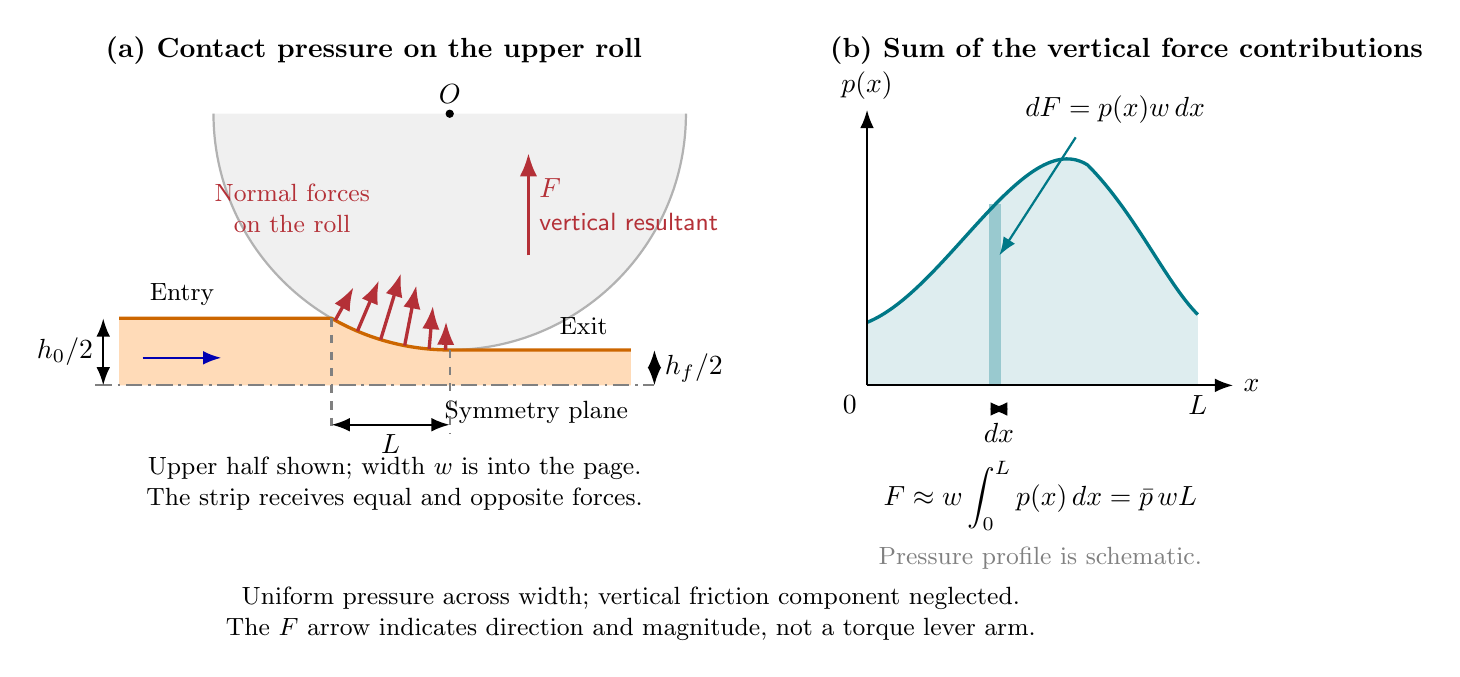
\begin{tikzpicture}[>=Latex,font=\sffamily,thick]
\definecolor{pressure}{RGB}{180,48,55}
\definecolor{area}{RGB}{0,120,135}
\pgfmathsetmacro{\hin}{3.45-3*cos(30)}
\node[anchor=west,font=\bfseries] at (-4.5,4.25) {(a) Contact pressure on the upper roll};
\path[fill=gray!12,draw=gray!60] (-3,3.45)
 arc[start angle=180,end angle=360,radius=3];
\path[fill=orange!28] (-4.2,0)--(-4.2,\hin)--(-1.5,\hin)
 arc[start angle=240,end angle=270,radius=3]--(2.3,0.45)--(2.3,0)--cycle;
\draw[orange!80!black,very thick] (-4.2,\hin)--(-1.5,\hin)
 arc[start angle=240,end angle=270,radius=3]--(2.3,0.45);
\draw[dash pattern=on 6pt off 2pt on 1pt off 2pt,gray]
 (-4.5,0)--(2.6,0);
\node[below,font=\small] at (1.1,-0.07) {Symmetry plane};
\draw[<->] (-4.4,0)--(-4.4,\hin) node[midway,left] {$h_0/2$};
\draw[<->] (2.6,0)--(2.6,0.45) node[midway,right] {$h_f/2$};
\draw[->,blue!70!black] (-3.9,0.35)--(-2.9,0.35);
\node[font=\small] at (-3.4,1.15) {Entry};
\node[font=\small] at (1.7,0.75) {Exit};
\fill (0,3.45) circle(1.5pt) node[above] {$O$};
% Inward radial arrows are forces exerted by the strip on the roll.
\foreach \ang/\len in {241/0.48,247/0.7,253/0.88,259/0.78,265/0.55,269/0.36}{
 \draw[->,pressure,very thick] ({3*cos(\ang)},{3.45+3*sin(\ang)})
 -- ({(3-\len)*cos(\ang)},{3.45+(3-\len)*sin(\ang)});
}
\node[pressure,align=center,font=\small] at (-2.0,2.25) {Normal forces\\on the roll};
\draw[->,pressure,very thick] (1,1.65)--(1,2.95)
 node[midway,right,align=left] {$F$\\\small vertical resultant};
\draw[dashed,gray] (-1.5,\hin)--(-1.5,-0.62);
\draw[dashed,gray] (0,0.45)--(0,-0.62);
\draw[<->] (-1.5,-0.5)--(0,-0.5) node[midway,below] {$L$};
\node[font=\small,align=center] at (-0.7,-1.25)
 {Upper half shown; width $w$ is into the page.\\The strip receives equal and opposite forces.};
\begin{scope}[shift={(5.3,0)}]
\node[anchor=west,font=\bfseries] at (-0.6,4.25) {(b) Sum of the vertical force contributions};
% Schematic pressure distribution; no claim of a solved pressure profile.
\path[fill=area!13] (0,0)--(0,0.8)
 ..controls(1,1.2)and(2,3.3)..(2.8,2.8)
 ..controls(3.4,2.2)and(3.8,1.3)..(4.2,0.9)--(4.2,0)--cycle;
\fill[area!40] (1.55,0) rectangle (1.7,2.3);
\draw[area,very thick] (0,0.8)..controls(1,1.2)and(2,3.3)..(2.8,2.8)
 ..controls(3.4,2.2)and(3.8,1.3)..(4.2,0.9);
\draw[->] (0,0)--(4.65,0) node[right] {$x$};
\draw[->] (0,0)--(0,3.5) node[above] {$p(x)$};
\node[below left] at (0,0) {$0$};
\node[below] at (4.2,0) {$L$};
\draw[<->] (1.55,-0.3)--(1.8,-0.3);
\node[below] at (1.675,-0.35) {$dx$};
\node[align=left,fill=white,inner sep=3pt] at (3.15,3.5) {$dF=p(x)w\,dx$};
\draw[->,area] (2.65,3.15)--(1.68,1.65);
\node[align=center] at (2.2,-1.40)
 {$F\approx w\displaystyle\int_0^L p(x)\,dx=\bar p\,wL$};
\node[font=\small,gray] at (2.2,-2.2) {Pressure profile is schematic.};
\end{scope}
\node[font=\small,align=center] at (2.3,-2.9)
 {Uniform pressure across width; vertical friction component neglected.\\The $F$ arrow indicates direction and magnitude, not a torque lever arm.};
\end{tikzpicture}
\end{document}
